\chapter{Results}
\label{sec:results}
In this chapter, the performance of the network architecture of this work, its components and results of classifications are going to be presented.
Mainly it is focused on the results of the grouping mechanism for analyzing the information content of views of the same objects but with different color marks.
Furthermore, the impact of different color marks is examined.
First, the overall performance of the network is discussed.
Then, the grouping mechanism is evaluated with respect to the information content of views, followed by an examination of misclassifications.
There are several networks trained with an increasing number of classes of combinations of category and color classes for being able to compare and dedicate possible occurring effects.
It starts with multi-views of only a single category, in particular, bathtubs, with first $n_m=3$ different color marks.
Those related color classes include the raw object, a green color mark and a red one.
This is further increased to $n_m = 6$ color classes containing a green and red color mark, two green color marks, and two red color marks.
Finally, $n_c = 4$ category classes in total are classified including additional dressers, monitors and sofas.
Here an identical process of adding color marks is performed in the same order as before.
This leads to a total of nine networks, where the basic architecture stays the same and only the number of outputs or classes $n_y$, respectively, changes.
However, for testing different hyperparameters, more networks have been trained on the dataset with bathtubs and 3 color classes.
In the following the syntax \emph{\#categories-\#colors} refers to the corresponding trained network where each number corresponds to the number of  classifications of the class type.
That means, the 4-3 network, for example, classifies a combination of four category classes and three color classes.
Furthermore, the 0-3 network classifies only color classes of bathtubs, while the 4-0 network classifies only category classes with blank objects.
The classes that each network predict are summarized in \tabref{tab:network-classes}.
Every model is trained for 20 epochs on the training set with a batch size of $m_b=8$.
Each batch element contains $n_v=12$ rendered views of an object.
The initial learning rate is set to $\gamma=0.0001$.
Furthermore, the dropout probability of layer 6 and 7 is specified as $0.5$ during training, which matches the AlexNet configuration.
Otherwise this layer is ignored, hence, is assigned a dropout probability of $0.0$.
Any dataset samples presented or predicted belong to the test set, thus, on data the network is not trained on.
This means, the training and test set contain the same classes, either category or color, but different data samples.
Each network is only trained once due to a lack of time, hence, all presented results refer to a particular training process and are not averages of several ones.
\begin{table}[]
\centering
\caption[Classification classes of each network]{Classification classes of each network. The notation follows \emph{\#categories-\#colors}.}
\label{tab:network-classes}
\begin{tabular}{l|ccccccccc}
               & \multicolumn{1}{l}{0-3} & \multicolumn{1}{l}{0-4} & \multicolumn{1}{l}{0-5} & \multicolumn{1}{l}{0-6} & \multicolumn{1}{l}{4-0} & \multicolumn{1}{l}{4-3} & \multicolumn{1}{l}{4-4} & \multicolumn{1}{l}{4-5} & \multicolumn{1}{l}{4-6} \\ \hline
Blank          & x                       & x                       & x                       & x                       &                         & x                       & x                       & x                       & x                       \\
Green          & x                       & x                       & x                       & x                       &                         & x                       & x                       & x                       & x                       \\
Red            & x                       & x                       & x                       & x                       &                         & x                       & x                       & x                       & x                       \\
Green-Red      &                         & x                       & x                       & x                       &                         &                         & x                       & x                       & x                       \\
Green-Green    &                         &                         & x                       & x                       &                         &                         &                         & x                       & x                       \\
Red-Red        &                         &                         &                         & x                       &                         &                         &                         &                         & x                       \\ \hline
Category classes & 0                       & 0                       & 0                       & 0                       & 4                       & 4                       & 4                       & 4                       & 4                      
\end{tabular}
\end{table}

\section{Overall Performance}
\label{sec:results-overall}
\section{View to Group Classification}
\label{sec:results-grouping}
Because the grouping mechanism supplies the core functionality of the network architecture it is evaluated first.
Even if the overall performance would yield satisfiable results, but the grouping mechanism would fail the original intention, it would need to be revised.
In contrast, if the results of the network are not satisfiable, the grouping algorithm could be the cause.

The easiest case for evaluation is a single object category with three material features.
Here the network only needs to find views with a material for assigning them a high discrimination score.
It is supposed, that those views have the highest scores of all views and, hence, are members of a group with a high weight.
Views where no material is seen, should have a score close to zero because the final prediction cannot rely on them at all.
Thus, this configuration is the most interpretable one.
The group dividing for the 0-3 network is shown in \figref{fig:grouping-0-3}.
Each number below a view refers to its score.
The text above views shows the group index with its corresponding weight.
All views appear in ascending order by their score.
Hence, all subsequent views are part of a group until another group is mentioned.
\begin{figure}
	\centering
	\begin{subfigure}{\textwidth}
		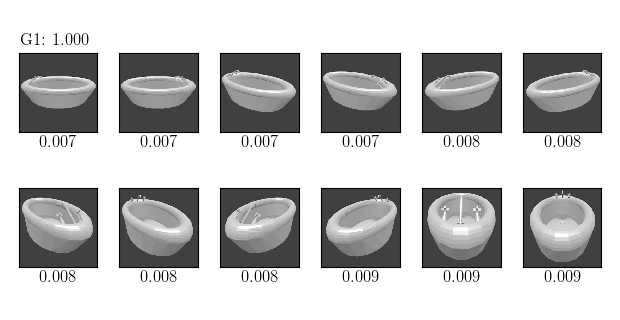
\includegraphics[trim=10 20 10 20, clip]{images/mn-sl-0-3-20/bathtub_0107_0_grouping.png}
		\caption{Blank}
		\label{fig:grouping-0-3-blank}
	\end{subfigure}
	\begin{subfigure}{\textwidth}
		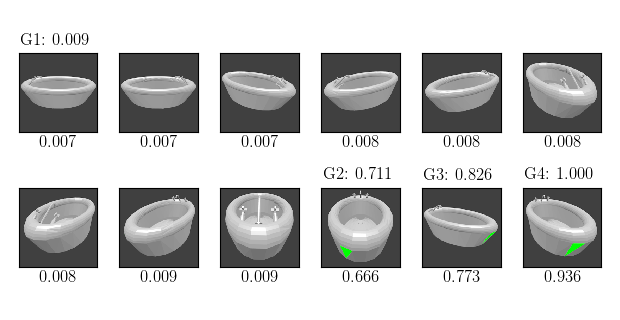
\includegraphics[trim=10 20 10 20, clip]{images/mn-sl-0-3-20/bathtub_0107_1_grouping.png}
		\caption{Green material}
		\label{fig:grouping-0-3-green}
	\end{subfigure}
	\begin{subfigure}{\textwidth}
		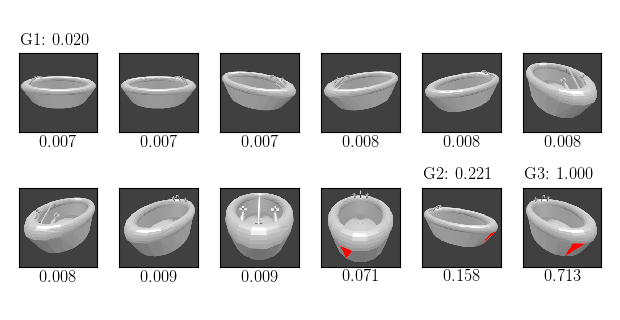
\includegraphics[trim=10 20 10 20, clip]{images/mn-sl-0-3-20/bathtub_0107_2_grouping.png}
		\caption{Red material}
		\label{fig:grouping-0-3-red}
	\end{subfigure}
	\caption[Grouping in 0-3 network]{Grouping in 0-3 network}
	\label{fig:grouping-0-3}
\end{figure}
In \figref{fig:grouping-0-3-blank} a blank object is classified.
Hence, every views is similar discriminative, due to no available colored material.
Thus, the view scores are almost identical.
Those little changes presumably depend on a different weight initialization and would even out after more training epochs.
Although the scores are very low, the views are fully taken into account because they all belong to the same group with a weight of 1.
However, in this particular case, a normalization of the group weight is not necessary.
Without one the group weight would be $w_G = 0.0079$, thus, decreasing the shape descriptor enormously, but the network would learn that a descriptor close to 0 represents a blank object.
The decision rule would be, if the descriptor represents no feature, the objects show no feature.
With the classification of more categories, though, this is not possible anymore, because a very small descriptor cannot just represent any blank object, but the object category class.
If there are two objects, for example, and only one view each shows a different feature with a small discrimination score, they would be divided into two categories.
Without a normalization, all views would pretty much account to the same amount to the shape descriptor.
Hence, the weights in the fully-connected layers for each specific present feature needs to be very large.
With normalization, however, the group with one view is much higher weighted than the not discriminative views.
Hence, normalization kind of removes noise, i.e. not discriminative views, that could influence the prediction unfavorably.
\figref{fig:grouping-0-3-green} and \figref{fig:grouping-0-3-red} show the expected result.
The views showing the material feature are by far the top-rated views referring to their score.
It looks like, that the network prefers the slightly tilted vertical edge with a feature to its right for recognizing material features.
This exact edge is not visible in the first view showing a feature, due to the change in perspective.
Due to the mesh representation of objects, all material features are triangles.
Perhaps the dataset contains more features following this shape than in rotated ones, hence, the network focuses on that correlation.
Moreover, both figures show exactly the same order.
This shows, that the weights for each color channel are optimized in the same direction.
However, the views with the green material are in a closer range compared to the ones with the red material.
The latter differs extremely.
The least discriminative view containing a material is closer to the not discriminative views than the discriminative ones.
Considering several different training sessions of this configuration, it is observed, that those scores of each material usually are similar to each other.
Hence, it is assumed, that a bad weight initialization caused this problem and a longer training would have evened it out.
Nevertheless, the group metric is at 1 for every material.
It should be noted, that always only a metric for the non-blank materials is given.
\begin{figure}
	\centering
	\begin{subfigure}{\textwidth}
		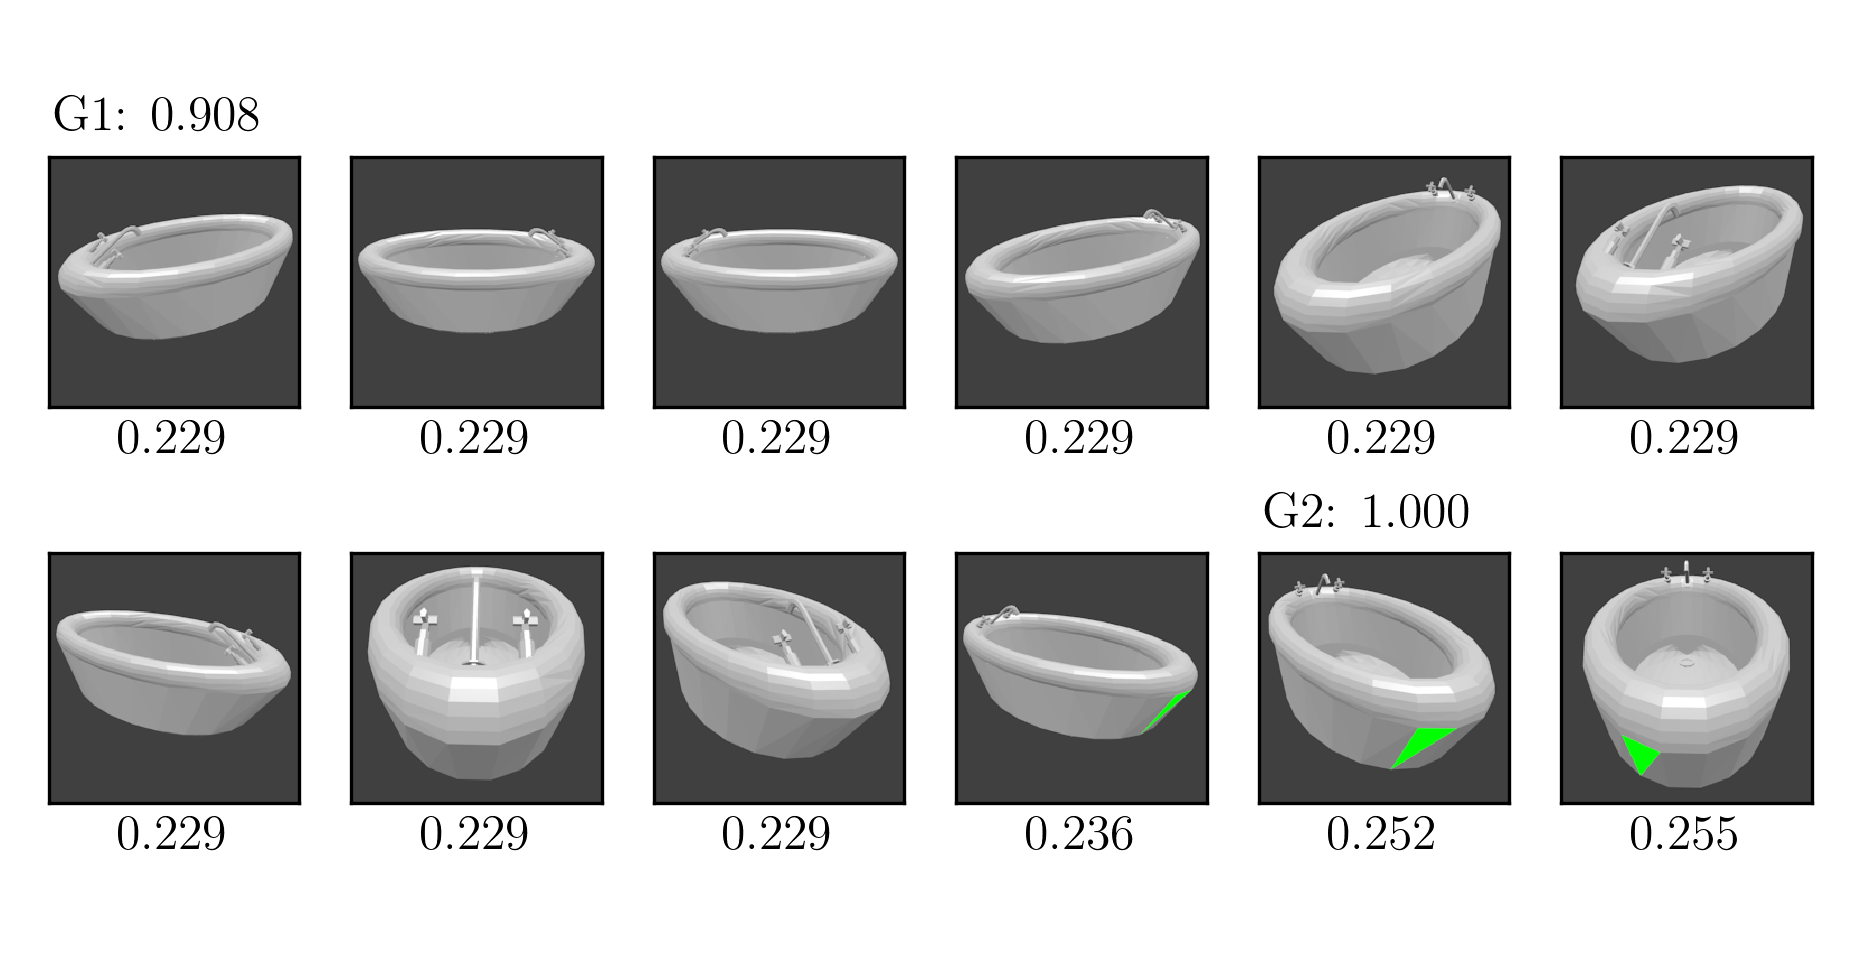
\includegraphics[trim=10 20 10 20, clip]{images/mn-sl-0-4-20/bathtub_0107_1_grouping.png}
		\caption{Green}
		\label{fig:grouping-0-4-green}
	\end{subfigure}
	\begin{subfigure}{\textwidth}
		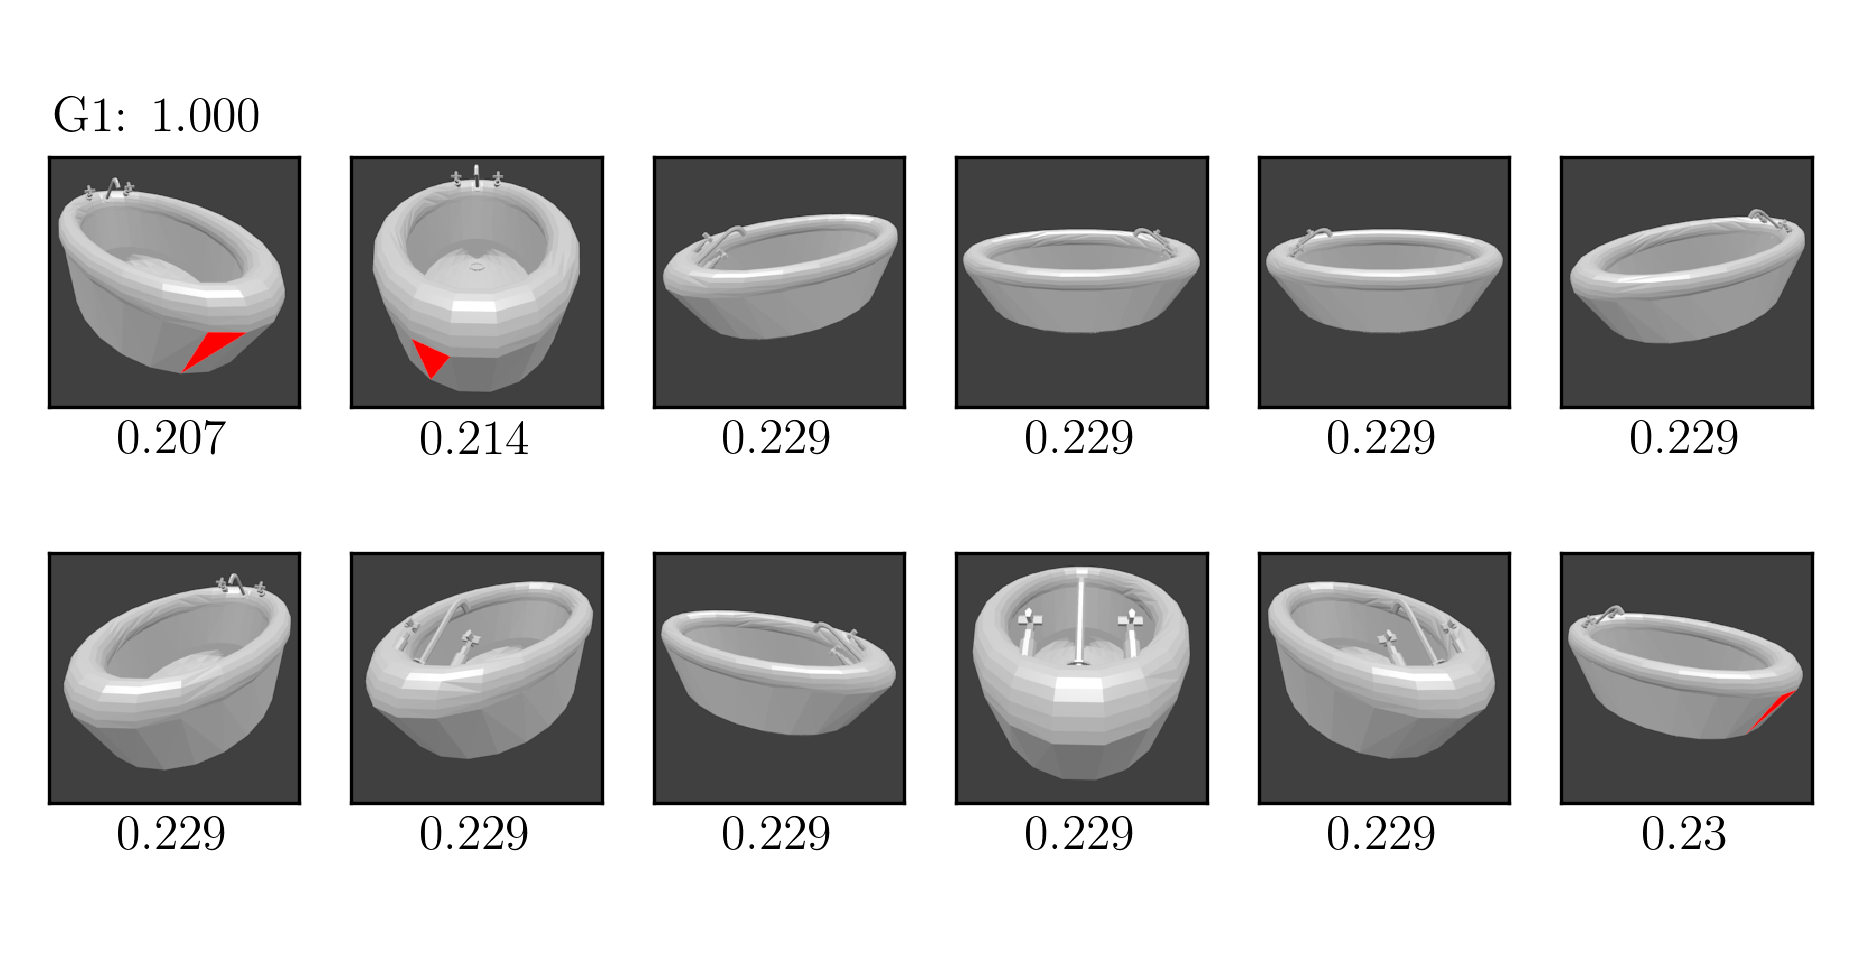
\includegraphics[trim=10 20 10 20, clip]{images/mn-sl-0-4-20/bathtub_0107_2_grouping.png}
		\caption{Red}
		\label{fig:grouping-0-4-red}
	\end{subfigure}
	\begin{subfigure}{\textwidth}
		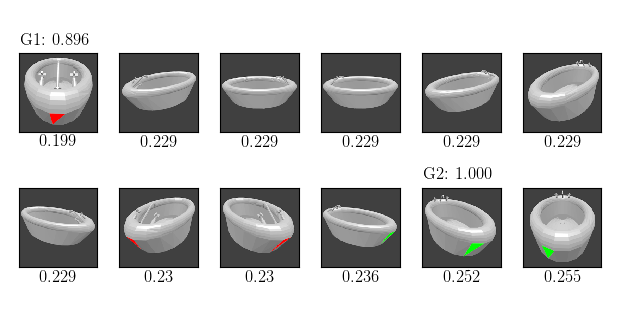
\includegraphics[trim=10 20 10 20, clip]{images/mn-sl-0-4-20/bathtub_0107_3_grouping.png}
		\caption{Green-red}
		\label{fig:grouping-0-4-green-red}
	\end{subfigure}
	\caption[Grouping in 0-4 network]{Grouping in 0-4 network}
	\label{fig:grouping-0-4}
\end{figure}
In \figref{fig:grouping-0-4} the grouping of the 0-4 network is shown, which additionally classifies green-red material features.
The divide of the blank object is omitted but all views have a score of 0.229.
Compared to the 0-3 network, this network finds different correlations, because the order of views is different.
Furthermore, not only the views with an available material are rated high like in \figref{fig:grouping-0-4-red}, but also the normal views like in \figref{fig:grouping-0-4-green}.
The reason is, that there could be two material features on a single object.
Hence, a view where a feature is supposed to be present is rated high, although it is missing.
This means, the discriminative information is the missing feature, thus, the view is more discriminative than it first seemed.
Therefore, a worse group metric than before is expected.
This is reflected by the values 0.735, 0.475 and 0.800 for each class.
The averaged group metric is 0.670.
This shows that the network prefers the green material as well because it is more often in the top group than the red one.
This is also seen in the red divide, where two of three material views are the least discriminative ones.
That suggests, that the red feature is treated as a sufficient criterion, while the green one is treated as the necessary criterion.
Moreover, it is not surprising, that the green and red features are mostly present in the top group.
\begin{figure}
	\centering
	\begin{subfigure}{\textwidth}
		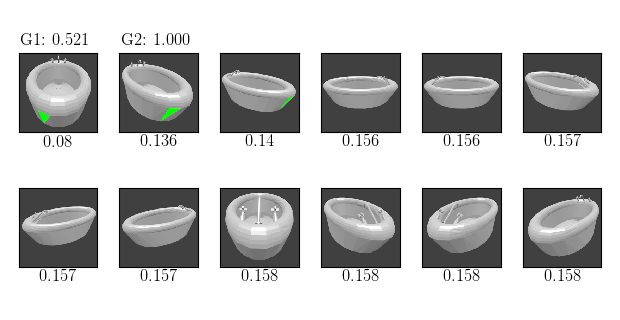
\includegraphics[trim=10 20 10 20, clip]{images/mn-sl-0-5-20/bathtub_0107_1_grouping.png}
		\caption{Green}
		\label{fig:grouping-0-5-green}
	\end{subfigure}
	\begin{subfigure}{\textwidth}
		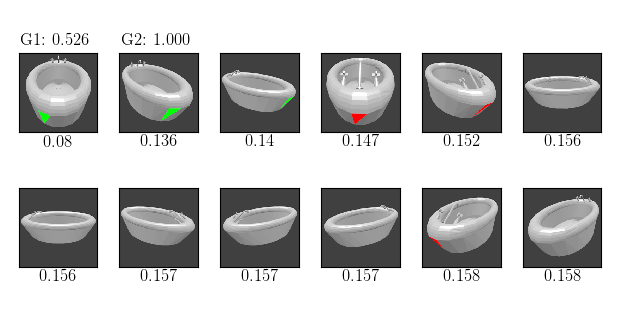
\includegraphics[trim=10 20 10 20, clip]{images/mn-sl-0-5-20/bathtub_0107_3_grouping.png}
		\caption{Green-red}
		\label{fig:grouping-0-5-green-red}
	\end{subfigure}
	\begin{subfigure}{\textwidth}
		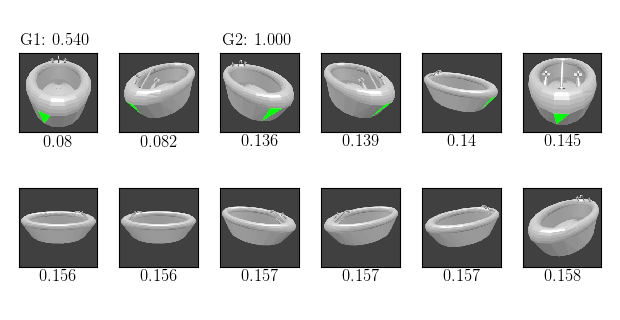
\includegraphics[trim=10 20 10 20, clip]{images/mn-sl-0-5-20/bathtub_0107_4_grouping.png}
		\caption{Green-green}
		\label{fig:grouping-0-5-green-green}
	\end{subfigure}
	\caption[Grouping in 0-5 network]{Grouping in 0-5 network}
	\label{fig:grouping-0-5}
\end{figure}
Next, the grouping for the 0-5 network is examined, that additionally classifies green-green features.
The important results can be seen in \figref{fig:grouping-0-5}.
The divide of the blank object is similar to the ones before.
There is only one group and the view discriminative scores are in a range of 0.156 and 0.158.
Not much changes for the divide of the red material.
The second view from earlier changes its position with the top view.
Moreover, the score of every view is decreased by about 0.07.
However, that the top view shows a red material is possibly for adding certainty for the classification with avoiding large weights.
For the green material, the material views are the least discriminative ones according to their score.
This is shown in \figref{fig:grouping-0-5-green}.
That effect must be due to the additional green-green feature.
An explanation could be, that the network now rates views by missing material features.
Hence, the shape descriptor becomes smaller the more features are available.
This theory is almost supported by the divide of green-red, that is shown in \figref{fig:grouping-0-5-green-red}.
Moreover, referring to the view scores, the views showing a green material have the exact same score than in the single green case.
However, the theory is changed in so far, that not the number of features is crucial, but rather that every material feature has a range in which it is classified.
Green materials are less discriminative than red ones and red ones are less discriminative than blank ones.
Using the green-green divide from \figref{fig:grouping-0-5-green-green} confirms this more.
The views with a green feature are less discriminative than the blank ones and also have a lesser score than the red ones in the earlier cases.
Thus, the shape descriptor is large, if no feature is visible, neutral if red ones are visible, slightly smaller if green ones are visible, small if both features are visible and very small if two green features are visible.
For this network, the group metrics are 0.419, 0.469, 0.768, 0.750 with an average of 0.601.
Those of each single feature and of each double feature are similar and the average is smaller than in the 0-4 case.
This supports the grouping theory even more in so far, that non-feature views are mainly members of the top group.
\begin{figure}
	\centering
	\begin{subfigure}{\textwidth}
		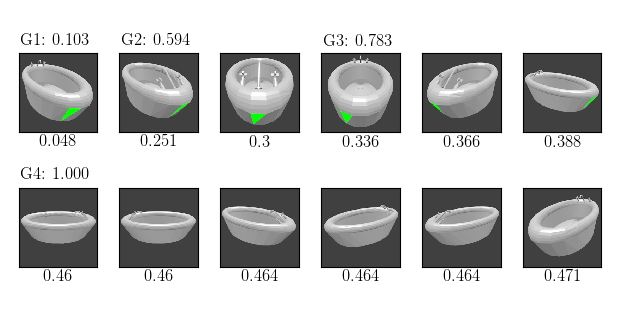
\includegraphics[trim=10 20 10 20, clip]{images/mn-sl-0-6-20/bathtub_0107_4_grouping.png}
		\caption{Green-green}
		\label{fig:grouping-0-6-green-green}
	\end{subfigure}
	\begin{subfigure}{\textwidth}
		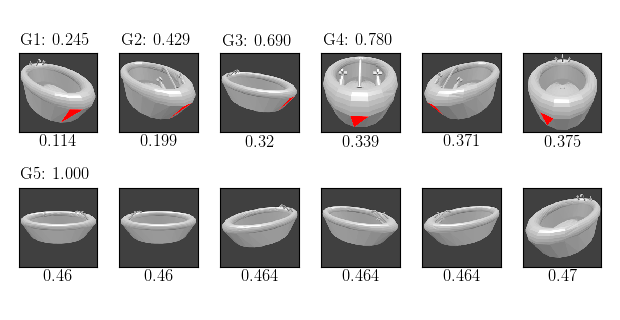
\includegraphics[trim=10 20 10 20, clip]{images/mn-sl-0-6-20/bathtub_0107_5_grouping.png}
		\caption{Red-red}
		\label{fig:grouping-0-6-red-red}
	\end{subfigure}
	\caption[Grouping in 0-6 network]{Grouping in 0-6 network}
	\label{fig:grouping-0-6}
\end{figure}
For having balanced evaluation results, red-red material features are added, yielding the 0-6 network.
Grouping blank views is almost identical to the earlier cases with the exception of view scores in a range of 0.46 to 0.472
The order of views for the green material has not changed notably.
However, an additional group is created and the scores of the views with a visible feature changed to 0.336, 0.048 and 0.388.
The remaining scores are in a range of 0.46 to 0.472 which matches the blank case.
In the red material case, the 0-5 top view is now the third-to-last.
Hence, all views showing materials are the least discriminative ones with scores of 0.106, 0.313 and 0.358.
The remaining views have identical scores to the other material cases.
Moreover, all of those views are divided into four groups.
In comparison, the green material and the red one have similar view scores, where the scores of the blank views are identical.
For the green-red case, all views not showing a material are more discriminative than the ones showing one.
This matches almost the grouping in the 0-5 network, but with five groups
The top group only contains non-feature views.
Furthermore, the scores of views with a green feature have the same score than in the single green feature case.
However, this is applicable to the views with red features.
This is due to the fact, that in this case, the second optimal face is colored red, hence, there are no comparable red faces.
For the green-green and red-red case, that are shown in \figref{fig:grouping-0-6}, the divide is almost identical.
The first one uses four groups the second five.
Though the view scores are similar, it is noticeable, that compared to each different colored feature in the green-red case views with a now green feature are less discriminative than views with a now red feature.
Although, both times the general score is higher.
Fortunately, this does not debunk the assumed theory of the group mechanism.
The corresponding group metric scores are 0.217, 0.253, 0.420, 0.381, 0.504 with an average of 0.355.
Their distribution is as expected, but with smaller values than in earlier networks.
This is due to the larger number of groups and the higher diversity of non-feature views to feature-views.

For a full understanding of the grouping mechanism, it needs to be examined, if the assumed theory is still valid if additional categories are classified.
This is done in the same order of number of classifications as with only material features.
First, the 4-0 network is evaluated.
It is supposed, that similar views like opposite perspectives of a symmetrical object are divided into the same group because they contain similar features.
For example, the views of the left and right side of a car look almost identical, due to having the same contours but in a mirrored direction.
\begin{figure}
	\centering
	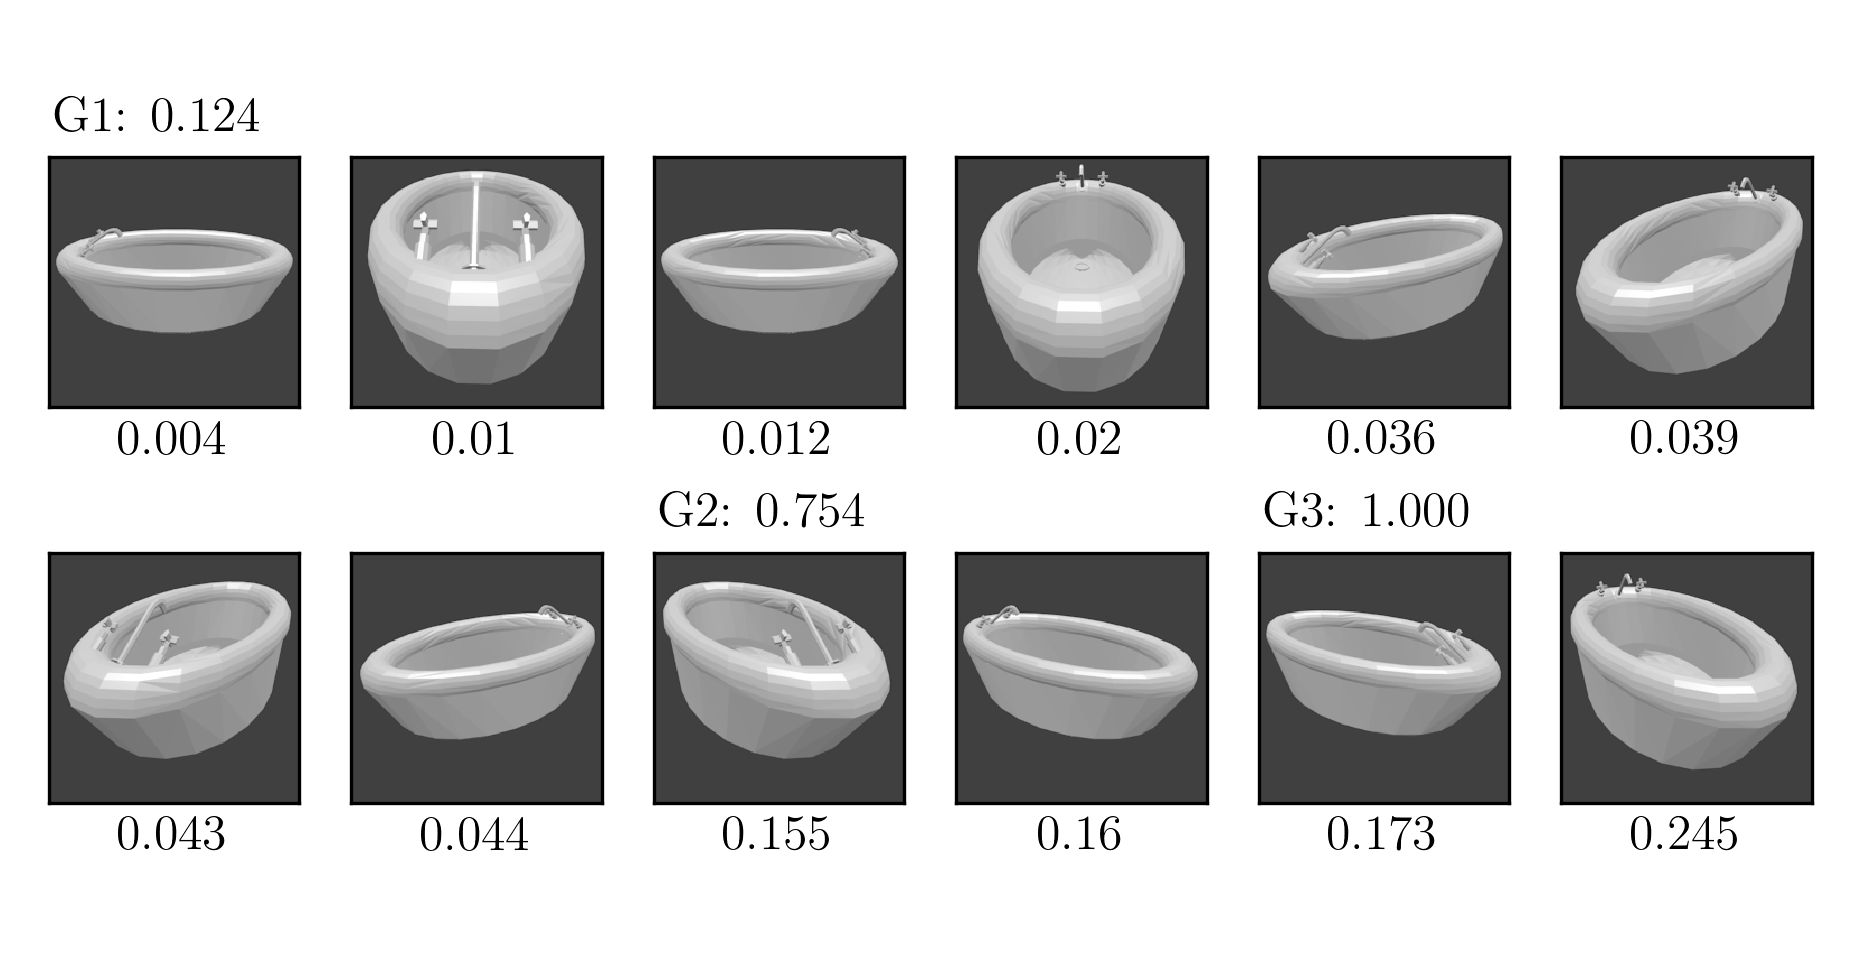
\includegraphics[trim=10 20 10 20, clip]{images/mn-sl-4-0-20/bathtub_0107_0_grouping.png}
	\caption{Grouping in 4-0 network}
	\label{fig:grouping-4-0}
\end{figure}
A grouping divide is shown in \figref{fig:grouping-4-0}.
It can be seen that the assumption is wrong.
Instead, the network prefers objects or features, respectively, that are diagonal from top left to bottom right.
This is validated by more predictions.
That such preferences are learned is already assumed from the 0-3 grouping.
The scores, however, are difficult to interpret.
For doing this it is necessary to compare all weights and activations, without achieving a real benefit, because the functionality of the grouping algorithm is already validated by using only materials.
Hence, the grouping for the remaining networks is briefly summarized.
Their divides are shown in \figref{fig:grouping-4-3}, \figref{fig:grouping-4-4}, \figref{fig:grouping-4-5} and \figref{fig:grouping-4-6}.
\begin{figure}
	\centering
	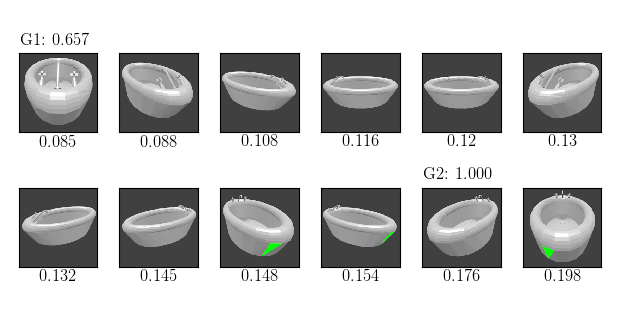
\includegraphics[trim=10 20 10 20, clip]{images/mn-sl-4-3-20/bathtub_0107_1_grouping.png}
	\caption{Grouping in 4-3 network}
	\label{fig:grouping-4-3}
\end{figure}
\begin{figure}
	\centering
	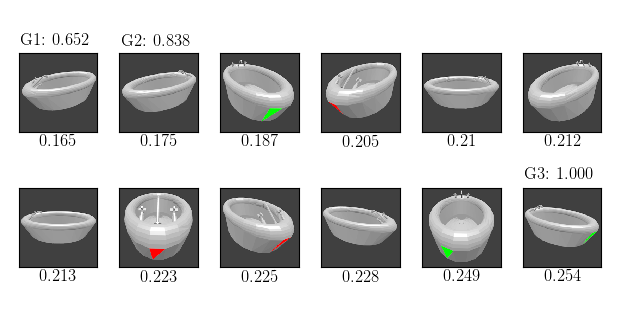
\includegraphics[trim=10 20 10 20, clip]{images/mn-sl-4-4-20/bathtub_0107_3_grouping.png}
	\caption{Grouping in 4-4 network}
	\label{fig:grouping-4-4}
\end{figure}
\begin{figure}
	\centering
	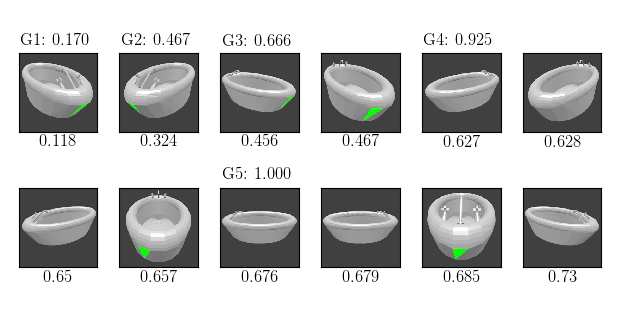
\includegraphics[trim=10 20 10 20, clip]{images/mn-sl-4-5-20/bathtub_0107_4_grouping.png}
	\caption{Grouping in 4-5 network}
	\label{fig:grouping-4-5}
\end{figure}
\begin{figure}
	\centering
	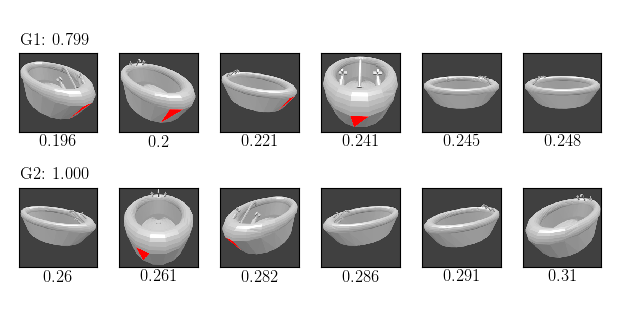
\includegraphics[trim=10 20 10 20, clip]{images/mn-sl-4-6-20/bathtub_0107_5_grouping.png}
	\caption{Grouping in 4-6 network}
	\label{fig:grouping-4-6}
\end{figure}
It can be seen, that each top group always contains at least one view with a visible feature.
Furthermore, the remaining ones are not necessarily discriminative, because depending on the number of materials it is more important to find features classifying the category.
Moreover, the more classes exist, the more groups are created.
That suggests, that the assumption from before, that shape descriptors of different classes are in different ranges, could be valid, because this way the network is more flexible in weighting views.
\section{Misclassified Predictions}
\label{sec:results-predictions}